% \begin{minipage}{0.49\textwidth}
%  \begin{tikzpicture}[scale=0.75]
%    \begin{axis}[ybar interval, ymax=6880,ymin=0, minor y tick num = 3, xlabel={CPU}, ylabel={Elapsed time (ms)}]
%      \addplot coordinates {(1,3963) (2,4639) (3,4763) (4,4790) (5,4934) (6,5090) (7,5207) (8,5326) (9,5727) (10,6880) (11,0)};
%     \end{axis}
%  \end{tikzpicture}
%  \caption*{ repeats kassian noupdate }
%\end{minipage}
%\begin{minipage}{0.49\textwidth}
%  \begin{tikzpicture}[scale=0.75]
%    \begin{axis}[ybar interval, ymax=6880,ymin=0, minor y tick num = 3, xlabel={CPU}, ylabel={Elapsed time (ms)}]
%      \addplot coordinates {(1,4471) (2,4750) (3,4789) (4,4824) (5,4964) (6,5312) (7,5359) (8,5366) (9,5373) (10,5518) (11,0)};
%     \end{axis}
%  \end{tikzpicture}
%  \caption*{ repeats randomized noupdate}
%\end{minipage}
\begin{minipage}{0.49\textwidth}
  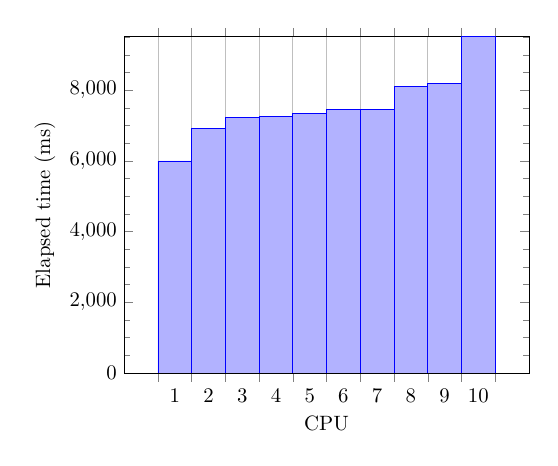
\begin{tikzpicture}[scale=0.75]
    \begin{axis}[ybar interval, ymax=9510,ymin=0, minor y tick num = 3, xlabel={CPU}, ylabel={Elapsed time (ms)}]
      \addplot coordinates {(1,5997) (2,6918) (3,7228) (4,7250) (5,7333) (6,7450) (7,7461) (8,8100) (9,8178) (10,9510) (11,0)};
     \end{axis}
  \end{tikzpicture}
  \caption*{Repeats  + kassian load balancing}
\end{minipage}
\begin{minipage}{0.49\textwidth}
  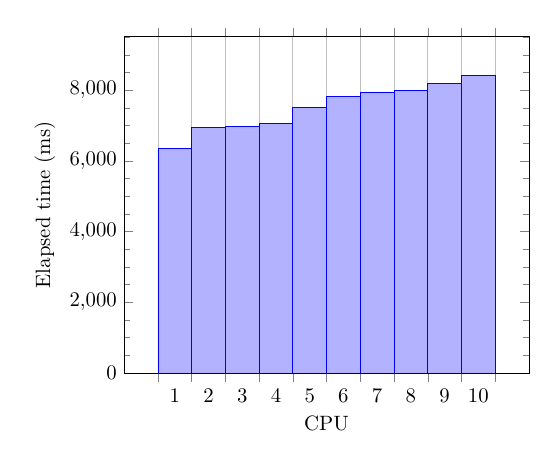
\begin{tikzpicture}[scale=0.75]
    \begin{axis}[ybar interval, ymax=9510,ymin=0, minor y tick num = 3, xlabel={CPU}, ylabel={Elapsed time (ms)}]
      \addplot coordinates {(1,6339) (2,6934) (3,6976) (4,7048) (5,7510) (6,7819) (7,7948) (8,7987) (9,8199) (10,8424) (11,0)};
     \end{axis}
  \end{tikzpicture}
  \caption*{Repeats + randomized load balancing}
\end{minipage}